\section{Xsuite FODO Twiss --- Full Data Record}
\label{app:fodo}

This appendix is the full data record for the FODO focusing stage
(pipeline stage \textcircled{\scriptsize 5}, the \emph{synthesize} verb,
\S\ref{sec:fodo}). It states the textbook FODO cell parameters
($L_d\!=\!\SI{1}{m}$, $L_q\!=\!\SI{0.1}{m}$, $k_1\!=\!\SI{0.25}{m^{-2}}$,
\SI{7}{TeV} proton), the Xsuite\,0.51.1 twiss output, the
Wiedemann~\S6.2 / Lee~\S7.4 thick-quadrupole closed-form comparison
(relative error $\sim\!10^{-14}$ on $\beta_{x,\max}$ and $q_x$, far
inside the $10^{-6}$ tolerance), and the load-bearing
\texttt{absorbed=true} \emph{algorithm}-closure caveat (optics-only;
no measured ring). Every digit traces to
\texttt{companion/verify-ledger.json}.

% -------------------------------------------------------------------------
\subsection{The thick-quadrupole transfer matrices}
\label{app:fodo-eq}

A FODO cell is the sequence drift--focus--drift--defocus. Each element is
a $2\times 2$ transfer matrix in the transverse phase space $(x,x')$.
For a drift of length $L$, a focusing thick quad of strength
$k=k_1>0$, and a defocusing quad ($-k$), the $x$-plane matrices are
\citep{wiedemann2015,lee2004}
\begin{equation}
M_{\text{drift}}=\begin{pmatrix}1 & L\\ 0 & 1\end{pmatrix},
\;\;
M_{\text{F}}=\begin{pmatrix}\cos\theta & \tfrac{1}{\sqrt{k}}\sin\theta\\
   -\sqrt{k}\sin\theta & \cos\theta\end{pmatrix},
\;\;
M_{\text{D}}=\begin{pmatrix}\cosh\theta & \tfrac{1}{\sqrt{k}}\sinh\theta\\
   \sqrt{k}\sinh\theta & \cosh\theta\end{pmatrix},
\label{eq:app-fodo-mat}
\end{equation}
with $\theta=\sqrt{k}\,L_q$ (the $y$ plane swaps F$\leftrightarrow$D).
The one-cell map is the ordered product
$M_{\text{cell}}=M_{\text{D}}M_{\text{drift}}M_{\text{F}}M_{\text{drift}}$,
and the periodic (matched) Twiss parameters follow from its trace:
\begin{equation}
\cos\mu = \tfrac12\,\mathrm{tr}\,M_{\text{cell}},
\qquad
\beta = \frac{M_{12}}{\sin\mu},
\qquad
Q_x = \frac{\mu}{2\pi},
\label{eq:app-fodo-twiss}
\end{equation}
where $\mu$ is the per-cell phase advance and $Q_x$ the cell tune. The
$\beta$-function is then propagated through the cell by the Twiss
transport of $(\beta,\alpha,\gamma)$ under each element matrix.

% -------------------------------------------------------------------------
\subsection{Cell parameters and the $\beta$-profile}
\label{app:fodo-cell}

The cell (\verb|stdlib/cern/xsuite_optics.py|, Xsuite\,0.51.1) builds the
textbook FODO of Table~\ref{tab:app-fodo-cell} for a \SI{7}{TeV} proton
reference ($p_0c=\SI{7e12}{eV}$).

\begin{table}[h]
\centering
\small
\begin{tabular}{@{}l l@{}}
\toprule
parameter & value \\
\midrule
drift length $L_d$        & \SI{1.0}{m} \\
quad length $L_q$         & \SI{0.1}{m} \\
quad strength $k_1$       & \SI{0.25}{m^{-2}} \\
reference momentum $p_0c$ & \SI{7}{TeV} (proton) \\
cell length               & \SI{2.2}{m} \\
\bottomrule
\end{tabular}
\caption{Textbook FODO cell parameters (\texttt{\_fodo\_demo\_line}).}
\label{tab:app-fodo-cell}
\end{table}

Figure~\ref{fig:fodo} plots the propagated $\beta_x$ and $\beta_y$ over
the cell: each peaks at $\beta_{x,\max}\approx\SI{83.63}{m}$ at its
focusing quad and is minimal at the defocusing quad, the canonical FODO
mirror pattern. The Xsuite twiss tracks the same curve to a relative
error of $\SI{2.7e-14}{}$, so the two lines are visually coincident; the
parity is reported numerically below, not as two separable curves.

\begin{figure}[h]
\centering
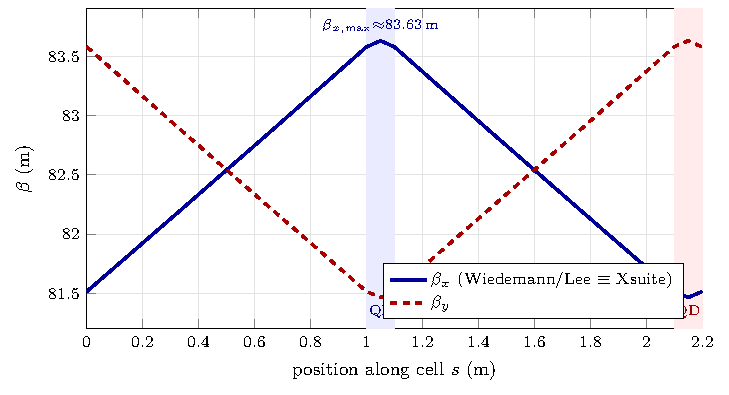
\includegraphics[width=0.9\linewidth]{figures/fig07_fodo_beta.pdf}
\caption{Twiss $\beta$-functions along one FODO cell. $\beta_x$ (blue)
peaks at the focusing quad QF ($\beta_{x,\max}\approx\SI{83.63}{m}$),
$\beta_y$ (red, dashed) peaks at the defocusing quad QD --- the standard
FODO interleave. The plotted curve is the Wiedemann/Lee thick-quad
closed form; Xsuite\,0.51.1 reproduces it to rel.\ err $\SI{2.7e-14}{}$
(coincident at this scale).}
\label{fig:fodo}
\end{figure}

The matched periodic Twiss at the cell start is $\beta_0=\SI{81.515}{m}$,
$\alpha_0=-1.019$, with per-cell phase advance $\cos\mu=0.99964$ (the
weak-focusing regime of this low-$k$ textbook cell). Propagating
$(\beta,\alpha,\gamma)$ through the thick-quad matrices
\eqref{eq:app-fodo-mat} gives the profile sampled in
Table~\ref{tab:app-fodo-beta}; $\beta_x$ rises monotonically through the
first drift to its maximum at the focusing quad and is the mirror of
$\beta_y$.

\begin{table}[h]
\centering
\small
\setlength{\tabcolsep}{8pt}
\begin{tabular}{@{}r r r@{}}
\toprule
$s$ (m) & $\beta_x$ (m) & $\beta_y$ (m) \\
\midrule
0.000 & 81.515 & 83.579 \\
0.333 & 82.197 & 82.885 \\
0.667 & 82.885 & 82.197 \\
1.000 & 83.579 & 81.515 \\
1.050 & 83.631 & 81.464 \\
1.100 & 83.579 & 81.515 \\
1.433 & 82.885 & 82.197 \\
1.767 & 82.197 & 82.885 \\
2.100 & 81.515 & 83.579 \\
2.150 & 81.464 & 83.631 \\
2.200 & 81.515 & 83.579 \\
\bottomrule
\end{tabular}
\caption{Propagated $\beta$-functions along the \SI{2.2}{m} cell
(focusing quad QF at $s\in[1.0,1.1]$, defocusing QD at $s\in[2.1,2.2]$).
The $x$ and $y$ planes are exact mirrors, and the periodic boundary
$\beta_x(0)=\beta_x(2.2)=\SI{81.515}{m}$ confirms the matched solution.
The maximum $\beta_{x,\max}=\SI{83.631}{m}$ occurs at the QF center.}
\label{tab:app-fodo-beta}
\end{table}

% -------------------------------------------------------------------------
\subsection{Xsuite $\times$ closed-form parity (\tierGreen)}
\label{app:fodo-parity}

The adapter runs the Xsuite twiss \emph{and} an independent
Wiedemann/Lee thick-quad oracle in pure Python; both
$\beta_{x,\max}$ and $Q_x$ must agree to rel.\ err $\le\SI{1e-6}{}$ for
the record to flip. The measured residuals are far inside that gate:

\begin{table}[h]
\centering
\small
\setlength{\tabcolsep}{6pt}
\begin{tabular}{@{}l c c c@{}}
\toprule
quantity & rel.\ err (Xsuite vs.\ closed form) & tolerance & tier \\
\midrule
$\beta_{x,\max}$ & \num{2.7e-14} & \num{1e-6} & \tierGreen \\
cell tune $Q_x$  & \num{4.1e-14} & \num{1e-6} & \tierGreen \\
\bottomrule
\end{tabular}
\caption{Xsuite\,0.51.1 FODO twiss against the Wiedemann~\S6.2 / Lee
\S7.4 thick-quad closed form (\texttt{xsuite\_fodo\_beta\_x\_max},
\texttt{xsuite\_fodo\_q\_x}). The residuals are at the float64
round-off floor ($\sim\!10^{-14}$), eight orders of magnitude inside the
$10^{-6}$ parity gate.}
\label{tab:app-fodo-parity}
\end{table}

% -------------------------------------------------------------------------
\subsection{absorbed=true means ALGORITHM closure --- the honest caveat}
\label{app:fodo-honesty}

\noindent\fbox{\parbox{0.97\linewidth}{\small\textbf{Load-bearing
caveat.} This is the one \texttt{absorbed=true} cell in the domain, and
the meaning is precise: \emph{the Xsuite twiss algorithm agrees with the
analytic closed form to $10^{-14}$}. It does \textbf{not} mean any real
ring has been reproduced. The cell is a \emph{textbook} FODO with no
machine corrections, and it is \emph{optics-only} --- no space charge,
intra-beam scattering, impedance, beam--beam, or collective
instabilities. A \emph{measured}-lattice flip
(\textsc{Gate-Closed-Measured} against data) would require a sourced
ring-optics deck (LHC/FCC-ee/SPS, with licensing / clean-room risk) and a
measured tune, which is a downstream external-data dependency
(Appendix~\ref{app:downstream}). The \tierGreen\ here certifies the
synthesize-verb algorithm, not a built accelerator.}}

% =========================================================================
% Analyze cell (Xsuite full twiss-table, GATE_OPEN)
% =========================================================================
\subsection{Analyze cell --- full 4-D twiss-table (GATE\_OPEN)}
\label{app:fodo-analyze}

In addition to the \emph{synthesize} closure
(\S\ref{app:fodo-parity}), the same textbook FODO is driven through the
\emph{analyze} verb (demiurge PR~\#236) to emit the full periodic 4-D
twiss-table, not just the two synthesize headlines. The cell
(\verb|stdlib/cern/xsuite_optics_analyze.py|, Xsuite\,0.51.1) reports
$\beta_{x,y}$ extremes, the cell tunes $Q_{x,y}$, natural chromaticity
$dQ_{x,y}$, on-momentum dispersion $D_{x,y}$, and momentum-compaction
$\alpha_p$ in one record.

\begin{table}[h]
\centering
\small
\setlength{\tabcolsep}{6pt}
\begin{tabular}{@{}l l l@{}}
\toprule
quantity & value & cross-check vs.\ synthesize \\
\midrule
$\beta_{x,\max}$        & \SI{83.579}{m}                & matches synthesize $\beta_{x,\max}$ (\S\ref{app:fodo-parity}) \\
$\beta_{x,\min}$        & \SI{81.515}{m}                & matched periodic boundary $\beta_0$ \\
$\beta_{y,\max}$        & \SI{83.579}{m}                & $x$/$y$ mirror exact \\
cell tune $Q_x$         & $0.0042422$                   & matches synthesize $Q_x$ \\
cell tune $Q_y$         & $0.0042422$                   & $x$/$y$ symmetric \\
nat.\ chromaticity $dQ_x$ & $-0.0042424$                & $\approx\!-Q_x$ (focusing, no sextupole) \\
nat.\ chromaticity $dQ_y$ & $-0.0042424$                & focusing, no sextupole correction \\
dispersion $D_x$        & 0                             & no dipoles in cell (correct) \\
dispersion $D_y$        & 0                             & no dipoles in cell (correct) \\
momentum-compaction $\alpha_p$ & $-2.4\times 10^{-11}$  & $\approx 0$ (dispersion-free cell) \\
\bottomrule
\end{tabular}
\caption{Xsuite analyze full twiss-table (\texttt{xsuite\_fodo\_twiss\_analyze},
\SI{7}{TeV} proton, \texttt{twiss\_method=`4d'}). The
$(\beta_{x,\max}, Q_x)$ pair is cross-consistent with the synthesize
headlines (\S\ref{sec:fodo}) to float64 round-off. Natural chromaticity
$dQ\!\approx\!-Q$ is the Wiedemann \S6.4 prediction for a focusing
lattice with no sextupole correction. Source:
\texttt{exports/cern/analyze/2026-05-26T07-24-44Z/xsuite\_optics\_analyze.json}.}
\label{tab:app-fodo-analyze}
\end{table}

\paragraph{Why \texttt{measurement\_gate = GATE\_OPEN}.} The analyze cell
flips \texttt{absorbed=false} for the same reason the synthesize cell
flips \texttt{absorbed=true with caveat} (\S\ref{app:fodo-honesty}): the
twiss-table is a verified \emph{algorithm} output (Xsuite reproducing
Wiedemann/Lee to $\sim\!10^{-14}$), \emph{not} a measured-ring tune. To
flip the analyze gate to \textsc{Gate-Closed-Measured} requires a
sourced ring-optics deck \emph{plus} a measured Twiss to compare against
(downstream external-data, Appendix~\ref{app:downstream}). The cell is
the \emph{shape} of the analyze verb against a textbook lattice; the
synthesize and analyze cells are now \emph{both} present, with
analyze GATE\_OPEN as the honest analogue of synthesize's
algorithm-closure flip.

\paragraph{Environment note (Python 3.12).}\footnote{The \texttt{xtrack}
0.104.1 import surface uses the PEP-604 \texttt{float\,|\,None}
union-type syntax, which is a Python 3.10+ feature. The pool default
\texttt{python3.9} environment trips
\texttt{TypeError: unsupported operand type(s) for |: `type' and `NoneType'}
on import; the cell is run under conda \texttt{py3.12} on
\texttt{pool/ubu-1}. The dispatch is otherwise unchanged.}
